%-------------------------------------------------------
\section{Problema - Objetivos - Producción}
%-------------------------------------------------------
\subsection{Pregunta de Investigación}
\begin{frame}{Problema y Objetivos}{Pregunta de Investigación}
%-------------------------------------------------------
  \begin{block}{Problema de Investigación}
   \begin{itemize}
   \justifying
    \item<1->  ¿Cómo realizar el direccionamiento de dispositivos heterogéneos conectados en una red Ad-Hoc, basada en comunicaciones máquina a máquina, autoconfigurable independientemente de la cantidad de dispositivos involucrados? 
    \item<1->  Los procesos y técnicas a emplear deberán estar enfocadas a la escalabilidad, simplicidad y robustez deseada en implementaciones encaminadas a servicios con conexiones tipo máquina-máquina.
    \end{itemize}
  \end{block}
\end{frame}
%-------------------------------------------------------
\subsection{Objetivos}
\begin{frame}{Problema y Objetivos}{Objetivos}
%-------------------------------------------------------
  \begin{block}{Objetivo General}
    \begin{itemize}    
    \item Diseñar un modelo de direccionamiento IPv6 en redes Ad-Hoc basadas en comunicaciones tipo máquina-máquina. 
    \end{itemize}
  \end{block}
  %\pause
  \begin{block}{Objetivos Específicos}
    \begin{itemize}
    \justifying
        \item Modelar los principales requerimientos en la asignación de direcciones IPv6 para redes Ad-Hoc.
        \item Adaptar, mediante técnicas bio-inspiradas, un algoritmo clásico de asignación dinámica de direcciones IPv6 para una red Ad-Hoc de 10 nodos. 
        \item Definir tres métricas representativas acerca del desempeño, sensibles para el modelo de direccionamiento propuesto.
    \end{itemize}
  \end{block}
\end{frame}
%-------------------------------------------------------
\begin{frame}{Problema y Objetivos}{Objetivos} 
  \begin{block}{Objetivos Específicos}
    \begin{itemize}
    %\setcounter{enumi}{3}
    \justifying
        \item Diseñar al menos tres escenarios de simulación en un software determinado, para someter el modelo de direccionamiento a diferentes condiciones a las que se podría enfrentar en una implementación real.
        \item Evaluar el desempeño del modelo planteado mediante simulaciones analizando las métricas definidas durante la ejecución de la tesis.
    \end{itemize}
  \end{block}
\end{frame}
%-------------------------------------------------------
\subsection{Producción Académica}
\begin{frame}{Problema y Objetivos}{Producción Académica}
%-------------------------------------------------------}
\centering

\includegraphics[width=0.7\textwidth,height=0.7\textheight,keepaspectratio]{Figures/COLCACI.JPG}\\
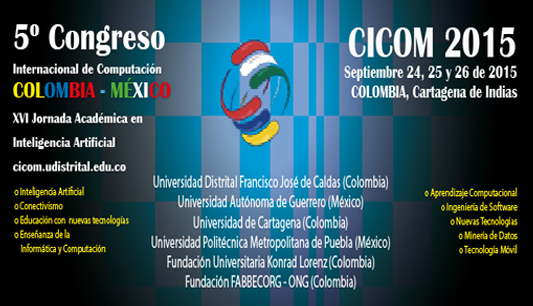
\includegraphics[width=0.6\textwidth,height=0.6\textheight,keepaspectratio]{Figures/CICOM.JPG}
\end{frame}